\documentclass[a4paper,12pt]{report}
\usepackage{titling}
\usepackage{graphicx}
\graphicspath{ {./images/} }
\DeclareGraphicsExtensions{.eps,.pdf,.png,.jpg}
\begin{document}
\begin{titlepage}
	\begin{center}
	%title
	\title{\Large Development of an OTA (Over the Air) Mobile Learning Telepresence Platform}
	\thetitle{\\}
	\textsc{\normalsize by\\}
	\author{\normalsize Kyle Galvin}
	\theauthor{\\}
	\normalsize\textsc{HBSc Computer Science, Lakehead University, 2013\\[0.5cm]}
	
	\textsc{A Thesis Submitted in Partial Fulfillment of the Requirements for the Degree of\\[0.5cm]}
	\textsc{MSC COMPUTER SCIENCE\\}
	\textsc{in the department of Computer Science\\[11.5cm]}




	\textsc{Copyright Kyle Galvin, 2013\\}
	\textsc{Lakehead University\\[0.5cm]}
	\textsc{All rights reserved. This thesis may not be reproduced in whole or in part, py photocopy or other means, without the permission of the author.}
	\end{center}
\end{titlepage}
\newpage
	\begin{center}
		\textsc{\LARGE Supervisory Committee\\[2cm]}
		\thetitle{\\}
		\textsc{\normalsize by\\}
		\theauthor{\\}
		\normalsize\textsc{HBSc Computer Science, Lakehead University, 2013\\[10cm]}
	\end{center}
	\textsc{\Large Supervisory Committee\\[0.5cm]}
	\textsc{Jinan Fiaidhi and Sabah Mohammed\\}
	\textsc{\emph{Supervisor}\\}
	\textsc{\emph{Co-Supervisor or Departmental Member}\\}
	\textsc{\emph{Departmental Member}\\}
	\textsc{\emph{Outside Member}\\}
\newpage

\tableofcontents

\chapter*{\centering Abstract}
Telepresence has been used in many forms in academia university for more than a decade by now as entities that help to maintain the relationship with learners and provide them with collaborative experiences without the expense of physical travel. However, the emerging technology has shifted its focus from the large class-room telepresence equipment’s to be scaled- down to mobile, wireless-networked telepresence products. With this technology shift, we are required to provide the learner with the ubiquitous ability to explore core learning contents deployed over the internet as well as to enable learners to interact with many other remote physical learning environments (e.g., Web environments, instructors, colleagues) through the use of mobile devices. This project aims at exploring this research area and to come with a solution for implementing a new type of learning objects that can be used over the air for telecollaboration and telepresence suitable for mobile platforms. 

\chapter{Lightweight Telepresence Technologies}

Microprocessors have shaped the world over the last century. Reducing in size over time exponentially, we are now able to achieve things that would have been unimaginable in the past. We can squeeze more bits per volume, transport more information and crunch more data each second than ever before. With this explosion of portability and connectivity comes a renaissance of technological growth that is unfolding before our eyes.

Density of information and computation as well as the speed of communication are at the core of modern digital technology, yet focusing on these features displays a very hands-on white box approach. There is also much to be learned with respect to the interaction between digital components and their environments, which could be considered more of a black box "I/O" style description. The interface a device supplies for others to interact with is just as important as the computational and communicative abilities the device has intenally to process the environment around it.

By extrapolating on current computational growth trends, we can imagine many applications in which technology will soon improve our every day lives. By studying these applications both mundane and whimsical alike, we are likely to find many exciting ideas which are attainable much more immediately than they first appeared.

Arthur C. Clarke once wrote "Any sufficiently advanced technology is indistinguishable from magic". Indeed many amazing discoveries can find roots in sci-fi and futuristic predictions which push the boundaries of our collective knowlege and explore the potential and logical conclusions of current technological progress. The most recent ideas which are moving from science fiction to science fact are telepresence and augmented reality. 

To introduce these ideas, I will borrow from the definitions others have supplied:
\begin{quotation}
Telepresence systems provide a human operator with the feeling of actual presence in a remote environment, the target environment. The feeling of presence is achieved by visual and acoustic sensory information recorded from the target environment and presented to the user on an immersive display.
	\begin{flushright}
		\cite{6094998}
	\end{flushright}
\end{quotation}

Likewise, an accurate and compelling description of augmented reality:

\begin{quotation}
AR is a variation of the more known concept of Virtual Reality Technology (VR), which is often defined as “the use of real-time digital computers and other special hardware and software to generate a simulation of an alternate world or environment, which is believable as real or true by the users”. VR technology creates an environment in which the user feels and seems to be moving inside a computer-created virtual world in the same way people move inside natural environment; while immersed in the virtual world, the user cannot perceive the real one which still surrounds him. On the contrary, AR allows the user to see the real world, augmenting it with superimposed virtual objects. In other words, while VR replaces reality, AR supplements it, creating an environment in which real and virtual objects harmonically coexist.
	\begin{flushright}
		\cite{5970856}
	\end{flushright}
\end{quotation}

\section{Emerging Mobile Technologies}
As microchip density increases, so does the mobility of computational and processing devices. While PDA and handheld gaming devices have been around for decades, the advance of cellular networks which allow for on-the-go personal telecommunications and widely dispersed access to internet services has really driven the shape and design of the current generation of mobile devices.

Smart phones and telecommunications aren't the only technology in this arena, but they are certainly the largest and most influential. Other devices to consider when discussing telepresence devices are lightweight microprocessors and system on a chip designs. These devices can allow industry and hobbiests alike to create a wide array of telepresence hardware that is capable of interacting with the environment around it on another's behalf. In this case, we are now less bound by strict computational limits and are now merely bound by the sensors, motors, and analog/digital conversions available to read from (and interact with) the environment around us.

When we combine our new-found freedom to invent any sort of sensory device with our fully connected and always online 'internet of things', we can begin to explore and create all sorts of ideas that were inaccessable to the real-world and thus bound to the realm of fiction, futurism, and sci-fi.
\subsection{Microcontrollers \& customized System on a Chip (SoaC) components}

Microcontrollers have become the de-facto platform for lightweight, mobile, and miniaturized devices. Much of the power of microcontrollers has been achieved by clever specializations and optimizations of the CPU unit. By diverging from the Desktop model where raw power takes precedence over power consuption, there are now a variety of architectures and specialized components that are well-suited to mobility. In fact there is now a wide spectrum of hardware ranging from high performance to low power consumption. With server and desktop harware on one end of the spectrum, we have recently expanded the power efficient end with a range of miniaturized ARM general-purpose CPUs capable of of supporting a general-purpose operating system and related peripheral components in an extremely small enclosure. To continue down the spectrum we depart from a traditional operating system and move towards programmable integrated circuits (PIC) and pure-hardware components which perform more specialized tasks using even less space and power.

Because of this balance between portability and power, it is important to keep in mind the practical limitations on the applications a device can support. While a computationally demanding task such as image processing, we are unlikely to get satisfactory results with a PIC controller, yet the current generation of ARM controllers which are recently emerging are just beginning to practically handle these tasks.

An interesting idea to consider is delegation of the heavy processing to a more capable device. However, this strategy simply moves the problem from the computational I/O boundaries of the device towards the networking I/O boundaries. To achieve practical results, we can use a hybrid approach by allowing the device to pre-process the data (assuming such a pre-processing can reduce the size of the raw data, preferrably an order of magnitude or more) before sending the derived result over the network to a more capable device.

Moving from our internal capabilities towards our external interactivity, we are capable of hooking up a wide array of sensors, displays, and feedback devices. From motors to spectroscopy sensors to audio capture and processing (and many, many more) the possibilities are limited only by the fidelity/accuracy of the sensors around us and our own creativity.

Before we wander into fanciful and eclectic descriptions of advanced robots and artificial intelligence which could easily be the plot of the next sci-fi thriller, we should take note of the challenges and limitations of today's robotic and so-called 'smart' devices. For example, to apply the concept of tele-robotics (where the telepresence user is represented and mimiced as a robotic avatar on the opposite end) the following challenges have been identified and discussed:

\begin{quote}
In this telepresence domain, as remote manipulators become more sophisticated and the tasks they undertake become more complex. Three main sensory obstacles to effective widespread use have been identified [15]:
	\begin{enumerate}
		\item The detection of sensory signals
		\item The feedback of real-time sensory information to the operator
		\item The presentation of this information in a form that can be easily detected, processed by the brain as a reflex action and responded to, since an excessive need for thought would detract from performance of the primary task.
	\end{enumerate}
	\begin{flushright}
		\cite{540147}
	\end{flushright}
\end{quote}

Aside from end-to-end synchronization and operator awareness, the question of usefulness and usability must also be addressed. Applicability has been fomrmally described as follows:

\begin{quote}

The main objective of tele-robotics has been to develop methodologies for the control of robots at remote sites by human users at local sites. Tele-robots are suitable in certain situations such as:
\begin{enumerate}
\item The robot must operate in environments that are hazardous to human health.
\item The robot must operate at a scale that is much smaller or larger than the human size and scale.
\item The robot must operate in a location where it would be too costly for the human to be present (in terms of budget, timing requirements, and human safety).
\end{enumerate}
	\begin{flushright}
		\cite{726589}
	\end{flushright}
\end{quote}

It begins to become clear that tele-robotics is not an idea that would lend itself to any situation. The reduction in fidelity we introduce by using a proxy or avatar robot is severe enough that we have only found successful use-cases in well-defined environments such as laboratories and factories where there are little or no unknown variables. Situations where there are people in close proximity to the robots are often too dangerous for the technology to be applied, and furthermore the decrease in the awareness a user would have with their remote surroundings makes the potential for interaction very limited. This barrier to adoption can be seen echoed in the following passage:

\begin{quote}
	Traditionally most robotic applications have involved the use of single static (non-mobile) manipulator platforms, with this technique being particularly suited to applications where the actual task is relatively well defined, the work volume is limited and safety considerations make even slightly “unexpected” motions totally unacceptable.
	\begin{flushright}
		\cite{540147}
	\end{flushright}
\end{quote}



\begin{quotation}{
	...the BCI collects the EEG brain activity and decodes the user's intentions, which are transferred to the robot via the Internet. The robot autonomously executes the orders using the navigation system (implemented with a combination of dynamic online grid maping with scan matching, dynamic path planning, and obstacle avoidance) or the camera orientation system. Thus, the shared-control strategy is built by means  of the mental selection of robot navigation or active visual exploration task-related orders, which can be autonomously executed by the robot.}
	\begin{flushright}
		\cite{6104414}
	\end{flushright}
\end{quotation}


The idea of presence fidelity can be considered a continuum. We can consider verbal descriptions and printed material on the low-fidelity end of the spectrum, while actual presence would be on the highest end. Our goal is to bring virtual telepresence farther along this continuum until it is as close to actual presence as possible \cite{726589}

\subsection{Mobile phones \& Cellular devices} When discussing mobile telepresence, the recent emergence of smart phones is undeniably the most important event to occur to date. In a learning environment they are indespensable for personal organization, time managment, and real-time updates. It has been stated by others that they can now allow students to ''...be informed of all necessary notices, assignment deadlines and supervisor advices during their busy schedule''. In fact, ''Mobile education is defined ... as any service or facility that supplies a learner with general electronic information and educational content that aids in acquisition of knowledge regardless of location and time.'' \cite{4469080}

\cite{6007847}
\section{Telepresence \& Real-Time communications}
\subsection{Audio/Video compression}
\cite{4297087}
\cite{4801602}

Within the context of mobile devices we need to consider not only the computational complexity and bandwidth consumption of video streaming, but the power consumption of the encoder as well.
\cite{5054795}
\subsection{Cellular network bandwidth flow \& optimization}

Network traffic can be prioritized using QoS (Quality of Service) classification. By prioritizing traffic types into real-time and non-real-time categories we can decrease the average latency on timing-critical services. By extending these concepts and including cooperative game theory strategies (by exploring Nash Bargaining Systems). A game theory strategy can be broken down into three components: Players, Strategies, and Interactions (or game utilities). If we can determine a metric for success in the context of each player, than we can create strategies which each player can use to interact with the system in a way which optimizes the collective success of all the players. Applied to bandwidth optimization, each network device is a player which utilizes a strategy for sharing the limited resources of the network.

The trend among wireless networks is an increased number of cells over smaller and smaller areas serving users. By reducing this cell size, we introduce an increased number of hand offs when the user is mobile. When a user passes from the range of one operator to the next, this hand-off should not interrupt the user's communication. Because of this, our QoS strategies should include a percentage of bandwidth reserved for hand-off services. 

With many different use-cases and bandwidth categories our goal is to create a strategy which optimizes the usability of all devices on the network. By ordering our bandwidth categories by highest to lowest priority we can allocate each users traffic into their respective categories while also dynamically adjusting the maximum flow of each category to reflect (as well as prioritize) the immediate demand in real-time
\cite{5710522}
\cite{1300874}
\cite{1376696}
\subsection{Privacy}
\cite{4698190}
\cite{4471983}

With the advent of Location Based Services (LBS) it is becoming increasingly difficult to control the extent in which a users locational information is used. Mix networks use short-term psudo-anonymous names to mask the identities of participants. With this mechanism, it becomes much more difficult for an adversary to correlate which actions in the system were performed by which users of the system.
\cite{6270872}
\cite{freudiger2007mix}
\cite{1032602}
\subsection{Cloud Based Assisted Technologies}

With the advance of internet connectivity, it is rare that modern mobile cellular devices are offline. If we are constantly in communication by means of a global (universal) IP address, It follows that we can achieve two things which we previously could not. 

First, we can synchronize our local data with the data of others in real-time. This lends itself to instant news aggregation, social media, e-mail, instant messaging, and even VoIP technologies. This is not in itself extremely surprising as these features have existed in the scope of the desktop application since the dawn of always on high-speed broadband connections, but the ability to bring this to a widely distributed array of mobile devices brings the connectivity of our society (and the speed of information travel as a result) to an all new level.

Second, we can now outsource services which are not desired or capable of running on the mobile device to another computer. While this is typically (as of yet) a cloud service provider's machine, it is reasonable to consider that over time software will develop which allows users to host their own content from a simple always-on home computer which serves as a personal hub for content including but not limited to public social media, geosecure proxy access, private home surveillance, and data storage. By using strict private/public tags, and 'group' authentication on a server's data as well as RSS-style content aggregators, it should be possible to design a decentralized 'home cloud' service which can serve many useful purposes to a mobile user in the field.

\section{Digital identification and modeling}

As our current trend of minniaturized mobile networked devices continues, the ability to stream high definition real-time media from many simple cellular devices is beginning to unfold. With higher quality cameras emerging in consumer devices as well as faster network connnectivity emerging in the forms of 3G and 4G telecommunication services it is completely feasible (even today) to use two phones to achieve a long distance video conversation.

It is interesting to consider that if we can stream enough information between two points to effectively allow a user to 'see' and 'hear' what is in another location, then theoretically speaking we must have processed and moved (via the VoIP phone system) enough information about the two locations to effectively understand (to the same degree the two communicating people were capable) what is happening at each of the locations. We as humans don't think about the image processing we do on a daily basis. We take for granted the fact that, somewhere between the rods and cones of our eyes and the high-level understanding we have of our surroundings, a lot of information was processed, stored, and acted upon.

While the topic of Artificial Intelligence and Computer Vision is far from bridging this gap, impressive results have been found by re-thinking the ways we can facilitate enhanced modelling and identification techniques.

\subsection{Bar codes \& QR codes}
QR codes (or two-dimensional bar codes) can reference nearly anything. Ranging in size from 25x25 to 177x177, they are most often used to redirect a user to a URL containing anything from videos to product info to social media content \cite{6182398}
Basic compression is done using run-length coding, where sequences of identical values are replaced with a single instance of that value followed by the repetition count. \cite{6182398}
\subsection{RFID; NFC}
\cite{5340296}
\subsection{real-time digital modeling}

\subsubsection{Triangulation \& Accelerometer based Orientated Positioning}

If many radio-enabled devices (whether via wifi, bluetooth, gps, or other means) are within communication range, it is possible to use time-synchronized signals to triangulate the positions of the devices with respect to each other. If any of these devices were equipped with a GPS, it could communicate this information and allow neighbors to take their local position data (respective to each other) and place them globally.

If any of these devices were equipped with an accelerometer and a camera, it is theoretically possible to calculate a position and orientation vector for the camera, effectively letting the device give extremely precise descriptions of what region of space is being recorded. This information (spatial meta-data, as well as the raw audio/video data) can be combined with other similar information from the region in order to provide high-fidelity reconstructions of recorded events. This information can be further augmented by other sensory input such as spectroscopes, depth-sensors, and environment monitors.

Time-synchronization techniques are limited by the sample speed of the measuring apparatus' clock. Determining distance by means of the recieved signal strenth do not require a clock, however the distance cannot be deduced from the signal strength alone without a calibration phase which takes into account the variance of each device's radio signal.

\subsubsection{Stitching multiple images/videos together}
In cases where images are not aligned, unwanted artifacts can be produced. Color and lighting inconsistencies can also be introduced which would create an unbalanced effect. A lack of references and identifiable control points can also make it difficult to correctly position image fragments. \cite{4359344}

\cite{5397590}
\subsubsection{Depth matricies/maps for 3D imaging}
Depth imaging techniques have only previously existed in costly special-purpose applications. With the spread of large-scale production on Time-Of-Flight sensors (specifically, the Microsoft Kinect) the accessability and spread of these devices has grown considerably. Time-Of-Flight technology involves measuring the delay between sending and recieving an infared signal. With this information, triangulation techniques can be used to measure the depth between the device and the target. 

These devices have been designed with object recognition in mind and are not particularly suited for 3d scanning applications. Low resolution and a large amount of noise are certainly factors when re-purposing these technologies for scanning\cite{6296662} 
\subsection{Image recognition and classification}
Image recognition is a complex problem often approached with a neural network model or similar fuzzy categorical organizer. If RGB information is augmented with depth information we can achieve much better results than if we were to rely on RGB information alone.
\subsubsection{Vector Quantization}
\subsubsection{Uncertainty / Fuzzy Logic}
\subsubsection{Improved accuracy through domain-specific environments/contexts}
telepresence surgery model - live data can be collected, then used to simulate the procedure virtually. 
This effectively allows us to generate training programs which are extremely accurate within the domain of the live collected data.

Imagine a doctor in front of device operates instrumentation which performs surgery on a remote patient.
instrumentation includes a wide variety of I/O (controls and sensory output via microphone, video, and even tactic feedback)
Assume access to highly detailed descriptions of our I/O over the duration of many operations (live experience captures)
The challenge is to make a virtual model of the operating procedure in which the doctor can interact with a virtual patient in a way which is synonymous with the standard interactions they would encounter with a live patient.

The challenge is considered 'solved' when the doctor cannot differentiate between a live patient telepresence experience and a simulated patient telepresence experience
I call this challenge the "Telepresence Turing Test", and it can be applied to any activity or domain in which telepresence can augment.

This challenge has a few interesting unknowns.

How 'synonymous' with live data can we realistically make the experience?

What are the most important factors we need to capture in our training data? What instrumentation can best capture those factors?

From the training data (live experience captures), how can we best create and improve upon a simulation model?\cite{391769} 

\section{Identifying the Major Elements for a Lightweight Mobile Telepresence System}

Lightweight mobile telepresence systems is a rapidly-evolving concept. Traditionally we have been bound by heavy and cumbersome desktop hardware, high-latency, and low network throughput. As these barriers have been reduced and removed, we have begun to redefine what it means to be connected.

Always-Available network communication

Real-Time video streaming

Geolocational services

Screen sharing (also useful for remote presentation)

File sharing (p2p for reducing infrastructure and bottle necks)

User/Group management and authentication

\section{Summary}

In conclusion, we are capable of much more than what is currently offered in terms of increasing the fidelity of our telepresence systems. On top of the increase in raw information storage capabilities, improvements in sensors as well as interactive peripherals have reshaped the way we use technology. If current trends continue we will soon find ourselves in a high density and highly distributed network of minniature devices, both as stand alone technologies (such as currently emerging smart phones) as well as embedded into every day consumer objects (as is the case with RFID tagging, QR coded items, and micro-controller enabled electronics). With this emerging paradigm it becomes much easier for computers to identify and process the objects around them, leading the way to many new modelling and digitizing techniques.

\chapter{Design Document}

\section{Goals}

Mobile Telepresence device which can traverse flat open space.
Battery operated
An on board camera

A phone application which can view the camera and control the base device

A system used to aid in telepresence integration for the remote viewee

\section{Design}
\begin{itemize}
\item Telepresence device equipped with ARM board controller which drives servos
\item Telepresence device also equipped with webcam and microphone
\item Android (Platform agnostic?) device on the client side for viewing live video and audio from telepresence device
\item Client side android device capable of driving the telepresence device
\item Computer vision techniques gives the viewer extended interactions with the remote environment. 

\item For example, a QR code the telepresence device encounters can open the resource on the viewers mobile device
\item For example, facial tracking techniques can be used to alert the remote viewer when somebody has entered the frame

\item augmented data systems applied to telecommunications and mobile telepresence

\item tons of data is available everywhere. There are many types of data and ways to visualize them and helpful calculations that can be done.

\item 'live' real time data is becoming more dense. from traditional IRC to VoIP and video streaming, bandwidth has come a long way

\item This live data can be parsed and processed immediately upon arrival

\item if we can process useful derivitive information in real-time with a small enough (how small?) latency, we can act on the results in a real-time manner.

\end{itemize}
\section{Networking}

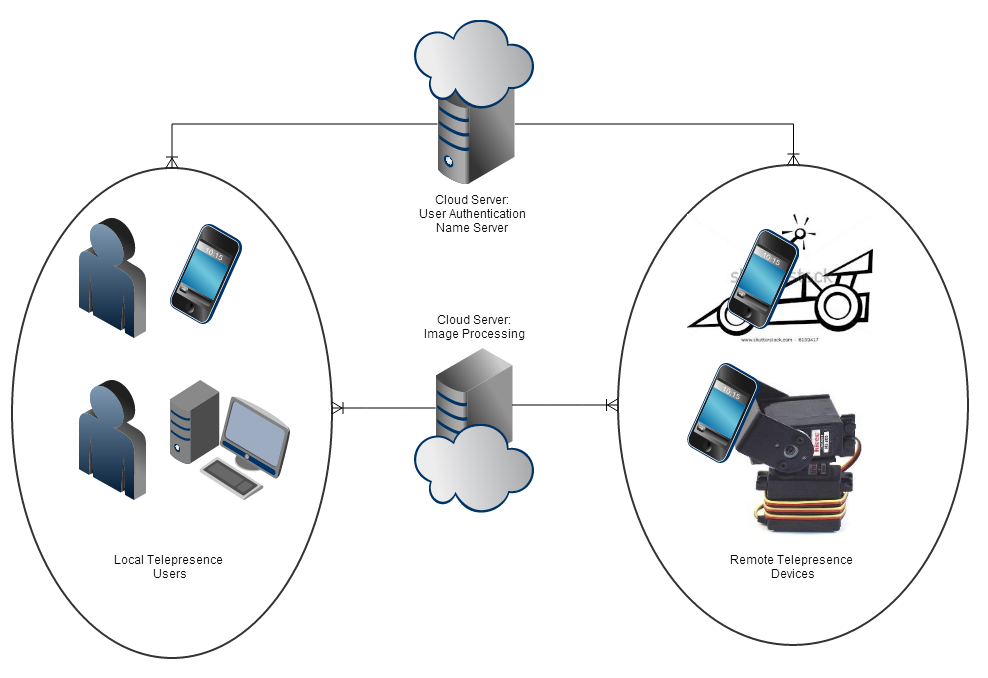
\includegraphics[width=12cm]{networkProfile_Labeled}

	\subsection{I/O Limitations}
		\begin{itemize}
		\item hardware needs high bandwidth, low latency
		\item how many video streams simultaneously?
		\item latency? Client\textless -\textgreater DSP\textless -\textgreater Hardware vs Client\textless -\textgreater Hardware direct
		\item performance trade-offs of doing DSP on robot or mobile device?
		\end{itemize}
		\subsubsection{optimizing performance}
			\begin{itemize}
			\item video compression
			\item audio compression
			\item measure opencv processing latency
			\item opencv gpgpu techniques
			\end{itemize}
	\subsection{Formal Grammar}
		develop a formal grammar to convey information from each module to the next
		\subsubsection{Commands}
			left,right,forward,backward
			toggle mute
			connect
		\subsubsection{Data}
			audio
			video
			augmented overlay (another video stream)
		\subsubsection{Multiple Roles}
			in some cases, data and commands are not divisible. eg: signal processing allows for commands to be encoded in video

\section{Hardware}
	The hardware component of the project is largely an exercise in manufacturing both structural and electronic devices. Many of the parts are off-the-shelf, while others will be hand crafted. The hardware for the project will consist of three parts. 

	The first part is a simple smart phone. While a web-enabled client could technically be used on a desktop (and in practice it could be) a mobile phone allows the user a great deal of flexibility and mobility. Assuming the user has access to a broadband connection, the client application should be simple enough to run on a small device. 
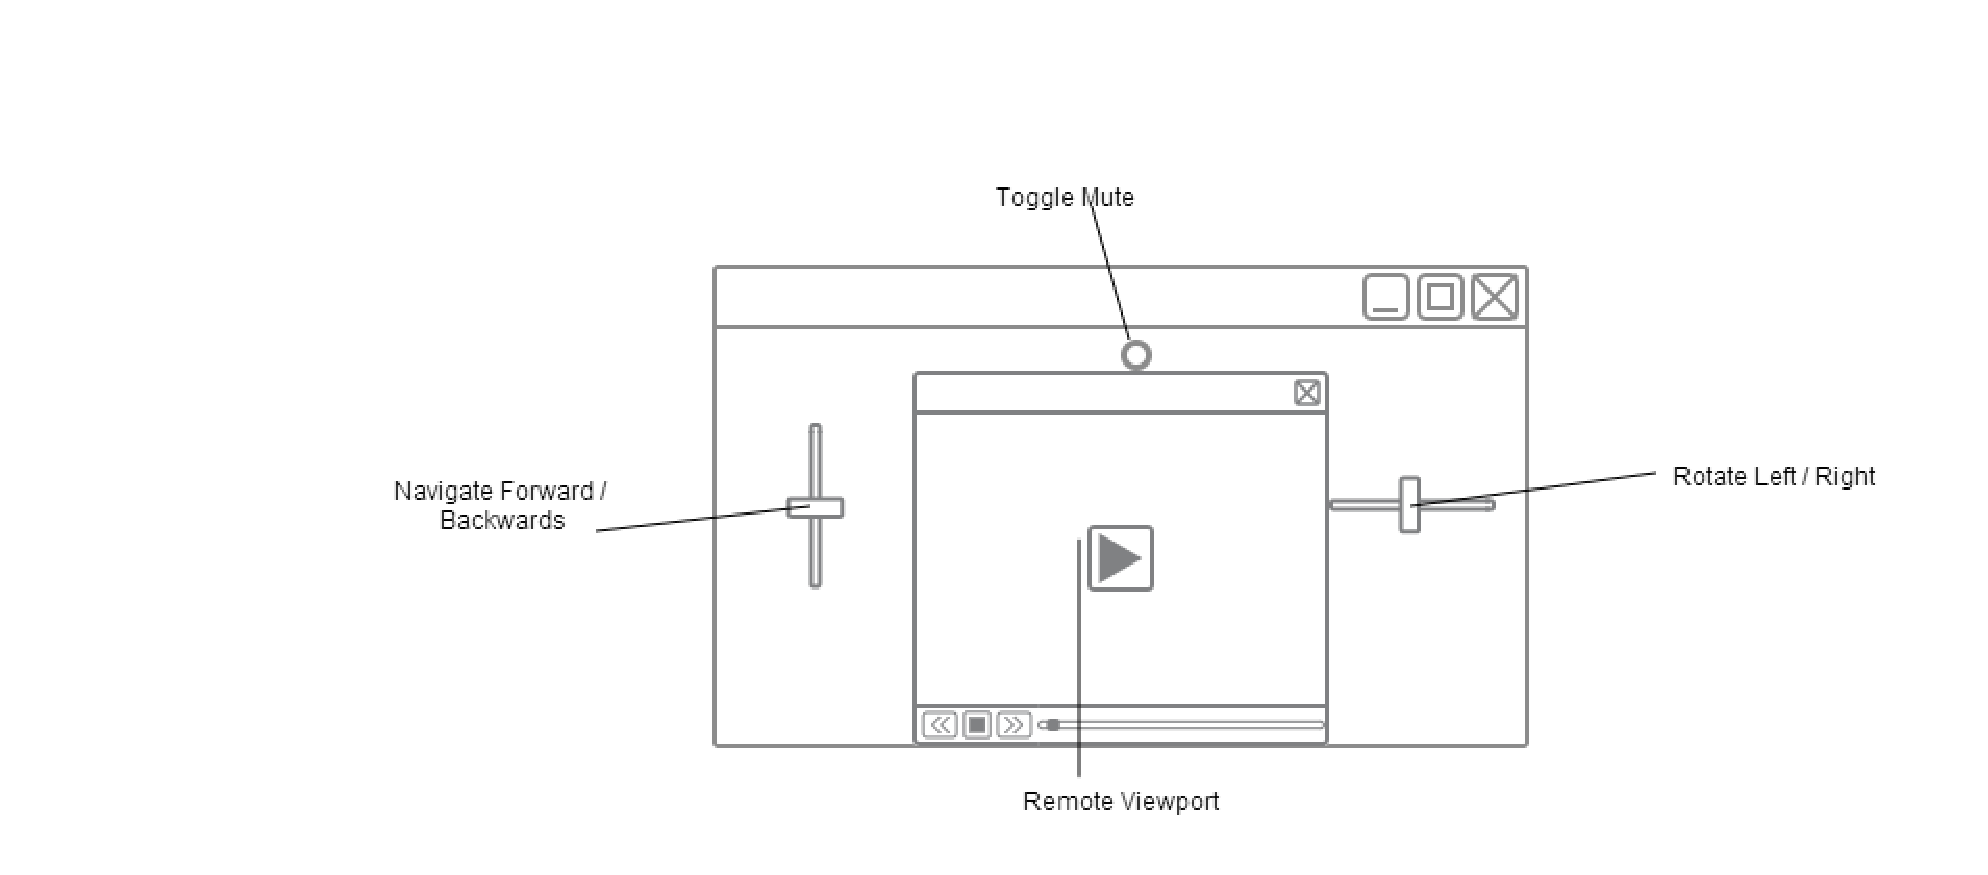
\includegraphics[width=12cm]{MobileGUI_Labeled}
\begin{itemize}
	\item smart phone client (android?IOS?) optionally desktop (if web app)
	\item Web stream in \textless video\textgreater element served by computer vision module
	\item touchscreen controls for left, right, forward, and reverse
	\item mute button turns speakers on and off
\end{itemize}

	The second part is the cloud server which does the signal processing. The computational requirements are not extreme, so a simple desktop computer will do for a laboratory environment.
\begin{itemize}
	\item cloud computation unit
	\item Basically a desktop computer with a GPU more capable than any of the embedded mobile devices
\end{itemize}

	The final part is the telepresence avatar.
\begin{itemize}
	\item vehicle
	\item weld steel chassis
	\item 2 servo drive
	\item raspberry pi piface interface acts as the controller
	\item pan / tilt? (maybe just tilt, tank already moves)
	\item camera
	\item standard webcam. 30fps streamed over wifi
	\item microphone
	\item built into camera
	\item speakers
	\item for speaking with remote users
	\item wifi
	\item usb wifi dongle.
\end{itemize}

\section{Digital Signal Processing}
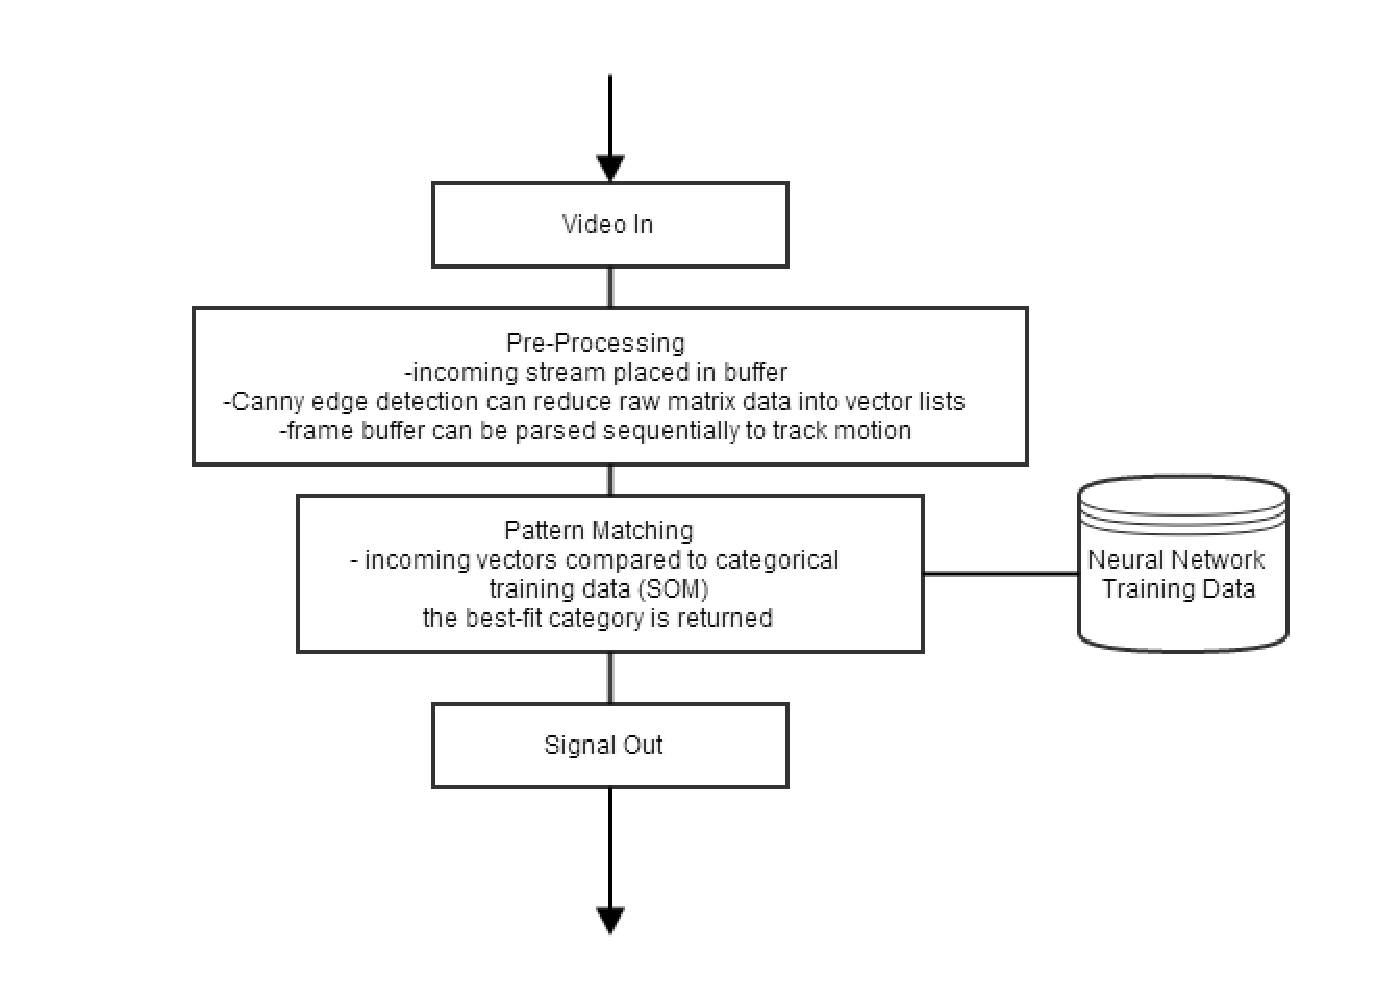
\includegraphics[width=12cm]{signalProcessing}
\begin{itemize}
	\item computer vision module
	\item raw video stream gathered from telepresence hardware
	\item video analyzed using computer vision and pattern recognition (opencv)
	\item client connected to this module will recieve events via the audio/video analyzer
	\item scripting language? HighGUI enough?
	\item client can also potentially recieve augmented audio/video data with the DSP module overlay
\end{itemize}
	
\subsection{Components}

Sensors/Input - generate data from the environment. Keyboard/Mouse are basic sensors. Video Cameras are more complex yet they are becoming extremely common. Many other sensors exist. GPS, microphone, accelerometer, etc.

Processor - consists of a three part pipeline:
	Data Extraction - reads the raw sensor data somewhere between the sensors and the client. Pre-processing can be done on the raw data, reducing it's size
	Pattern Recognition - the pre-processed data can be analyzed and compared against a database of models. If the data matches the models (within a degree of tolerance) than properties can be assigned to the data
	Action/Augmentation - As properties are discovered in the live data stream, they will trigger actions within the system. Actions can then be sent along with the raw data towards the client device which is capable of acting on the augmented stream

Client/Output - will recieve the real-time data along with augmented action events. Action events will be acted on.

Actions can get as complex as you like. For example, the client's device could initiate a video call if it detects a series of actions such as "a presenter is in the room and the presenter is speaking and the client has just raised their hand"


\bibliography{mastersthesis}
\bibliographystyle{alpha}
\end{document}
